\documentclass{article}
\usepackage{graphicx}
\usepackage{amsmath}
\usepackage{float}
\usepackage{amsthm}
\usepackage{fancyhdr}
\setlength{\headheight}{22.48724pt}
\usepackage[breaklinks]{hyperref}
\usepackage[margin=1in]{geometry}
\usepackage{listings}
\usepackage{xcolor}
\usepackage[scaled=0.85]{beramono} % Clean, modern monospaced font
\usepackage{booktabs}

\usepackage[T1]{fontenc}
\definecolor{codebg}{RGB}{250, 250, 250}
\definecolor{commentgreen}{RGB}{34, 139, 34}
\definecolor{keywordblue}{RGB}{0, 0, 205}
\definecolor{stringred}{RGB}{178, 34, 34}
\definecolor{numbergray}{RGB}{128, 128, 128}

\pagestyle{fancy}
\fancyhf{}
\fancyhead[L]{Maaz Mansuri, Fayella Fenton, Joshua Scallo, Gavin Palacios \\ RFR27 new member-10}
\fancyhead[R]{\thepage}

% Configure Listings for Arduino C/C++
\lstdefinestyle{arduinoStyle}{
    backgroundcolor=\color{codebg},
    commentstyle=\color{commentgreen}\itshape,
    keywordstyle=\color{keywordblue}\bfseries,
    numberstyle=\tiny\color{numbergray},
    stringstyle=\color{stringred},
    basicstyle=\ttfamily\footnotesize,
    breakatwhitespace=false,
    breaklines=true,
    captionpos=b,
    keepspaces=true,
    numbers=left,
    numbersep=7pt,
    showspaces=false,
    showstringspaces=false,
    showtabs=false,
    tabsize=2,
    frame=single,
    rulecolor=\color{lightgray}
}
\lstset{style=arduinoStyle}

\hypersetup{
    colorlinks=true,
    linktoc=section,
    linkcolor=blue,
}

\title{2027 Digital Precharge}
\author{Jeevan Shah}

\begin{document}
\begin{titlepage}
	\centering
	\vfill

	{\Huge \textbf{RFR27 16-Channel Temperature Monitor New Member Project-10}\par}

	\vspace{0.5cm}

	{\Large Rutgers Formula Racing\par}

	\vspace{0.5cm}

	{\large Maaz Mansuri, Joshua Scallo, Fayella Fenton, Gavin Palacios \par}
	{\large \today \par}

	\vspace{2.5cm}

	
\includegraphics[width=0.5\textwidth]{RFR EV Logo White Bolt - Black Letters - Red Body.png}

	\vfill
\end{titlepage}

\newpage

\tableofcontents

\newpage

\section{Revision Log}
\begin{tabular}{| c | c | c |}
	\hline
	Editor       & Date          & Revision \\
	\hline
	Maaz Mansuri & Oct. 12 2026 & Document Creation        \\
	\hline
    Maaz Mansuri & Oct. 15 2026 & Established outline of documentation and table of contents \\
    \hline
    Fayella Fenton & Oct. 15 2026 & Inserted Source Refs \\
    \hline
    Joshua Scallo & Oct. 17 2026 & Added schematic and hardware descriptions \\
    \hline
    Maaz Mansuri & Oct. 19 2026 & Completed firmware Design and added flowcharts for the circuit and the code \\
    \hline
    Joshua Scallo & Nov. 4 2026 & Updated schematic version and completed schematic design justifications.  \\
    \hline
\end{tabular}

\section{Purpose}
Create a 16-channel temperature monitor for the accumulator container and transmit pack thermal data over the I2C bus upon master query.

\section{Parties Involved}
\begin{tabular}{| c | c | c |}
	\hline
	Name        & Team Role                            & Report Role \\
	\hline
	Maaz Mansuri & Software & Author      \\
	\hline
    Joshua Scallo & Hardware & Author \\
    \hline
    Fayella Fenton & Hardware & Author \\
    \hline
    Vaanika Singla & Electronics Lead & Reviewer \\
    \hline
    Jeevan Shah & Electronics Lead & Reviewer \\
    \hline
\end{tabular}


\section{Hardware Design}

\begin{figure}[H]
    \centering
    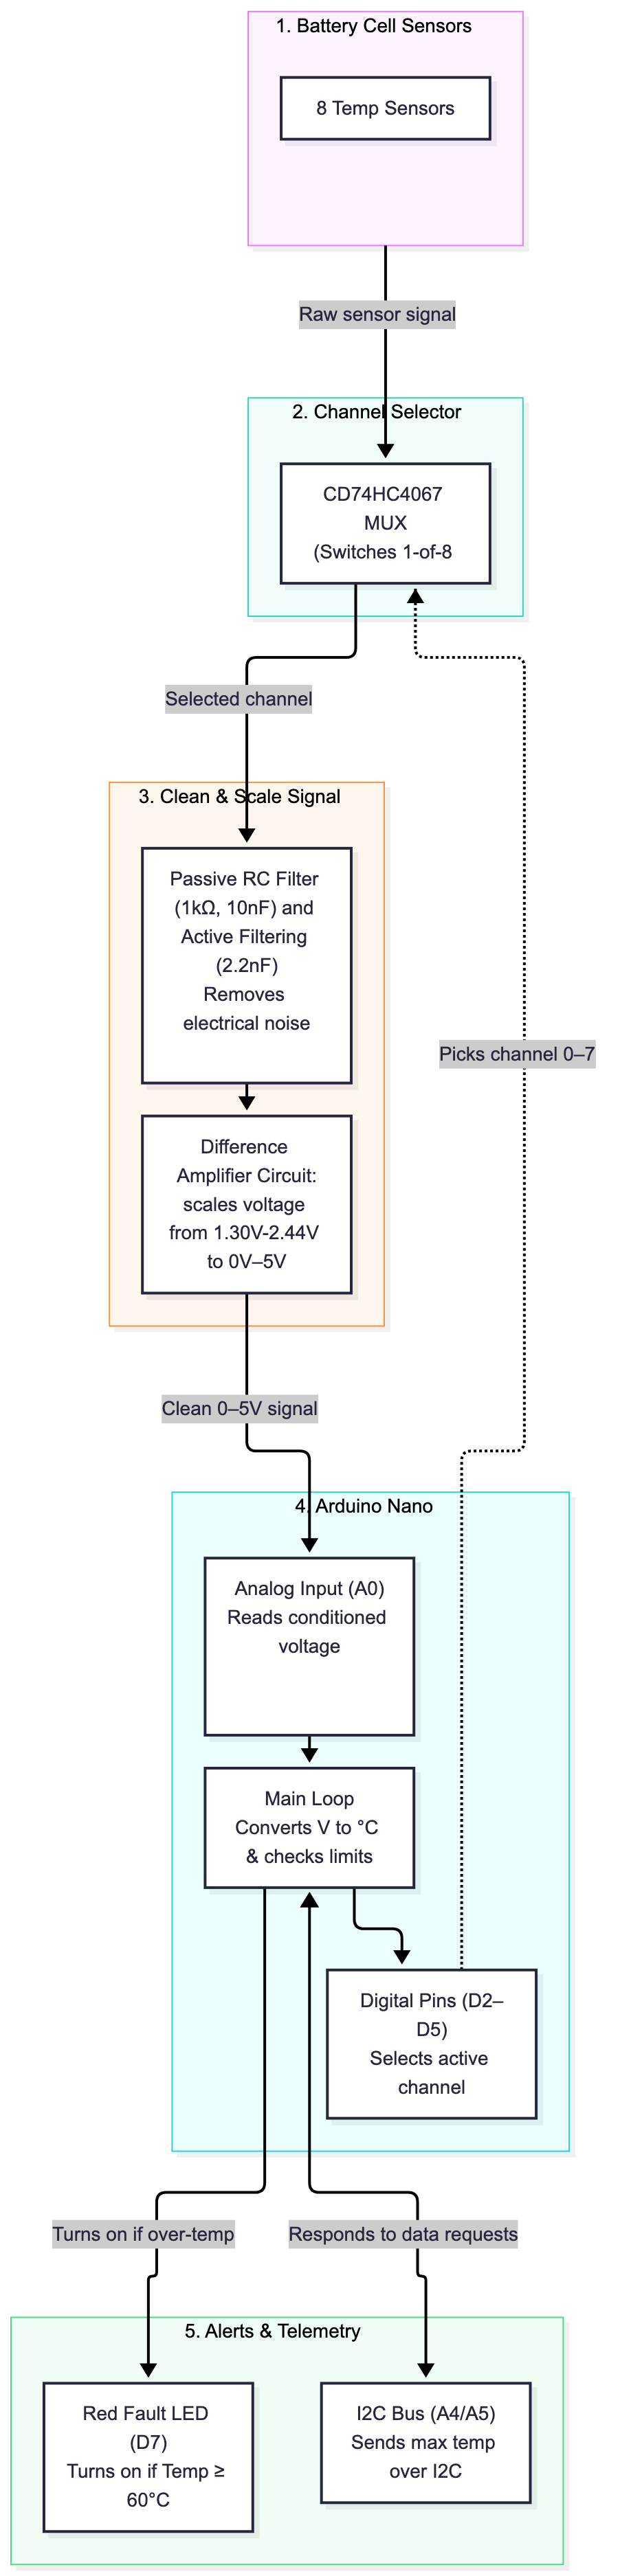
\includegraphics[height=0.65\textheight, width=0.85\linewidth, keepaspectratio]{circuitflowchart.png}
    \caption{Hardware System Signal-Flow and Architecture Diagram}
    \label{fig:hardware_flowchart}
\end{figure}

\begin{figure}[H]
	\centering
	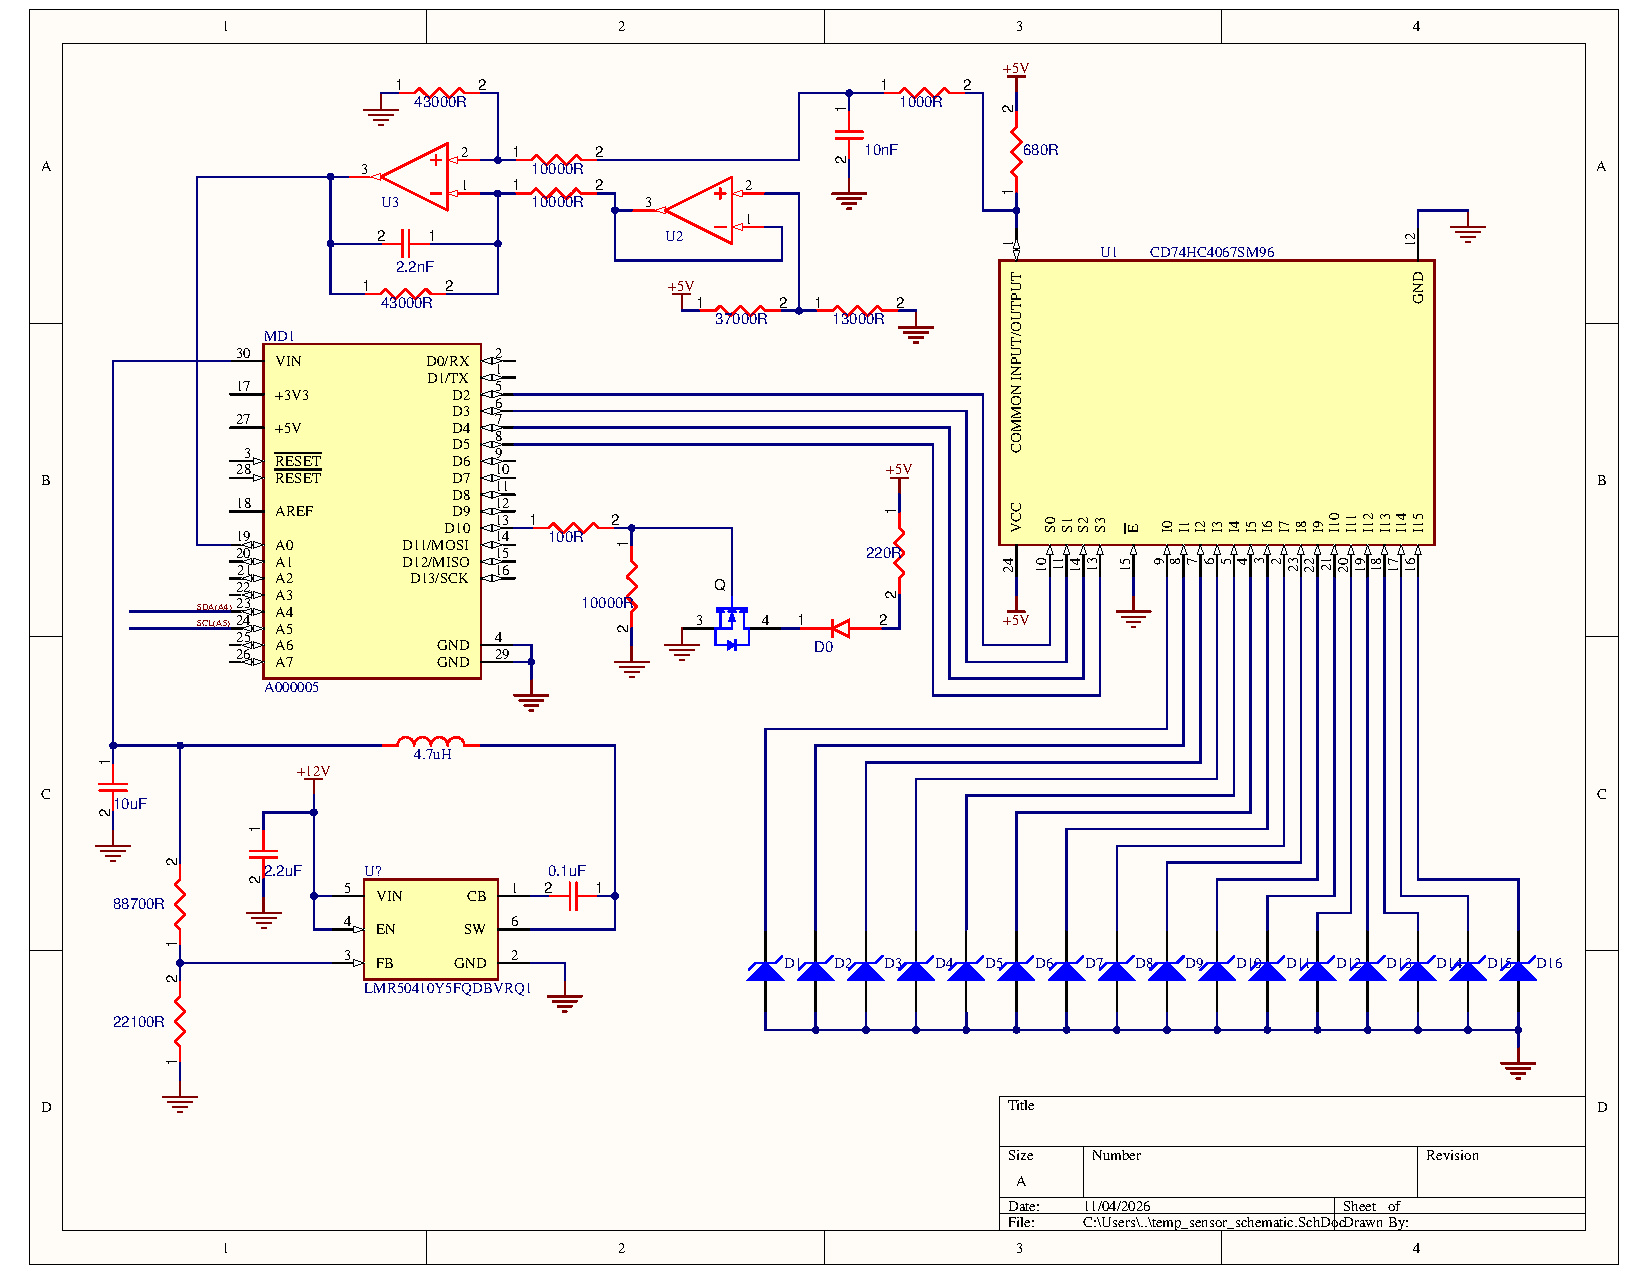
\includegraphics[width=\linewidth]{arduino_temp_sensor_v4.pdf}
	\caption{Schematic}
	\label{fig:arduino_temp_sensor_v4}
\end{figure}

\subsection{Introduction to Schematic Design}
Our schematic design contains 16 temperature sensors represented by zener diodes, a 16-channel multiplexer (CD74HC4067SM96), signal conditioning circuitry, an Arduino Nano, and a buck converter (LMR50410Y5FQDBVRQ1). This design allows the use of the Arduino Nano's onboard ADC to collect the voltage readings from each temperature sensor one by one with help from the 16-channel multiplexer. This is achieved by connecting each channel of the multiplexer to a temperature sensor reading. These channels are then controlled by the firmware in the Arduino Nano's D2-D5 pins, where each chosen output of the multiplexer is first conditioned, then sent to the A0 pin of the Arduino Nano, where the voltage is gathered and tested through the firmware. The MOSFET-controlled LED connected to the D10 pin then shines when the voltage reading interprets a temperature reading higher than 60 C.

\subsection{RC Filter}
\begin{itemize}
    \item RC filter's main intention is to smooth out the sharp changes from the MUX switching between channels.
    \item $1\,\text{k}\Omega$ resistor will act as a current limiter. The resistor value cannot be too high, or it will affect the difference amplifier's $10\,\text{k}\Omega$ resistance value and mess with its overall gain. 
    \item $10\,\text{nF}$ capacitor is chosen due to time constant ($\tau$).
\end{itemize}
\textbf{Cutoff Frequency:}
\[
f_c = \frac{1}{2\pi R C} \approx 15.9\,\text{kHz} \quad 
\]

\subsection{Difference Amplifier}
\textbf{Temperature Sensor Voltage-Temperature Outputs:}
\[
\begin{array}{rccc}
\text{Temperature:} & -40^\circ\text{C} & \longrightarrow 60^\circ\text{C} \longrightarrow & 120^\circ\text{C} \\
\text{Output Voltage:} & 2.44\,\text{V} & \longrightarrow 1.81\,\text{V} \longrightarrow & 1.30\,\text{V} \\
& (\text{min temp}) & (\text{target temp}) & (\text{max temp})
\end{array}
\]

\vspace{0.5em}
\noindent \textbf{Difference Amplifier Circuit Analysis:} \\
Intended to create a $0\,\text{V} - 5\,\text{V}$ output range from the temperature sensor readings ($1.30\,\text{V} - 2.44\,\text{V}$).

\noindent \textbf{Transfer Function:}
\[
V_O = \frac{R_2}{R_1} (V_{\text{MUX}} - V_{\text{REF}}) \quad \left(\text{where } \frac{R_2}{R_1} \text{ is gain } A\right)
\]
\[
5 = A(2.44 - 1.3) \implies A = \frac{5\,\text{V}}{1.14\,\text{V}} \approx 4.386
\]

\noindent Using standard resistor values:
\[
R_1 = 10\,\text{k}\Omega \quad \text{and} \quad R_2 = 43\,\text{k}\Omega
\]
\[
\frac{43\,\text{k}\Omega}{10\,\text{k}\Omega} = 4.3 \implies A = 4.3 \quad (\text{ideal gain is truncated down to avoid clipping above } 5\,\text{V})
\]


\subsection{Voltage Divider \& Buffer Op-Amp}
\textbf{Voltage Divider Calculation:} \\
We want $V_{\text{REF}} = 1.3\,\text{V}$:
\[
5 \left( \frac{R_2}{R_1 + R_2} \right) = 1.3\,\text{V}
\]
Using standard resistor values:
\[
R_2 = 13\,\text{k}\Omega \quad \text{and} \quad R_1 = 37\,\text{k}\Omega
\]

\vspace{0.5em}
\noindent \textbf{Buffer Op-Amp Analysis:}
\begin{itemize}
    \item Buffer op-amp will prevent \textbf{voltage loading}.
    \item Internal Thevenin resistance from $R_1$ \& $R_2$ of the voltage divider will affect the $R_1 / R_2$ ratio of the difference amplifier.
    \item Buffering will create a clone $1.3\,\text{V}$ (provided by $5\,\text{V}$) that is clean like a $1.3\,\text{V}$ battery.
\end{itemize}


\subsection{Active Filtering ($2.2\,\text{nF}$ Capacitor)}
\[
gain(f) = \frac{R_f}{R_{\text{in}}}
\]
\[
Z_F = \frac{R_f}{1 + j 2 \pi f R_f C_F} \quad \text{with } C_F = 2.2\,\text{nF}
\]
\[
f_0 = \frac{1}{2 \pi R_f C_F} \approx 1.682\,\text{kHz}
\]
\[
Z_f = 0\,\Omega \quad @ \quad f = 0\,\text{Hz}
\]
\[
Z_f = 43\,\text{k}\Omega \quad @ \quad f \approx 1.68\,\text{kHz}
\]
\begin{itemize}
    \item This means higher frequencies will short-circuit $R_f$, which will make the gain equal zero.
    \item This allows higher frequencies to be eliminated.
\end{itemize}

\subsection{Settling Time Analysis}

Settling time exists due to the time it takes for the filter's capacitors to charge/discharge every time the multiplexer switches channels.

\noindent Capacitor follows an exponential charging curve:
\[
V(t) = V_S \left(1 - e^{-t/\tau}\right) \quad (\tau \text{ is time constant})
\]
For an accurate reading from the 10-bit ADC on the Arduino, we need to consider the ADC resolution:
\[
\frac{1}{2^{10}} = 0.000977 = 0.0977\%
\]
To prevent sensor voltage reading overlap (crosstalk), the filter has to settle within $0.0977\%$ of its final value.

\noindent We need to find how many time constants are needed to reduce the error below $\frac{1}{2^{10}}$:
\[
e^{-t/\tau} = \frac{1}{2^{10}} \implies \ln\left(e^{t/\tau}\right) = \ln\left(2^{10}\right)
\]
\[
\frac{t}{\tau} = 10 \ln(2) \approx 6.93 \implies t \approx 6.93\tau
\]
To prevent errors, round up: $t = 7\tau$.

\subsubsection*{Hardware Settling Breakdown}
\begin{itemize}
    \item \textbf{RC Filter:}
    \[
    7\tau_1 = 7(1\,\text{k}\Omega \times 10\,\text{nF}) = 70\,\mu\text{s}
    \]
    \item \textbf{Active Feedback:}
    \[
    7\tau_2 = 7(43\,\text{k}\Omega \times 2.2\,\text{nF}) = 662.2\,\mu\text{s}
    \]
    \item \textbf{Total Hardware Settling Time:}
    \[
    70\,\mu\text{s} + 662.2\,\mu\text{s} = \underline{732.2\,\mu\text{s}}
    \]
\end{itemize}

\subsection{Verifying 1000Hz Sampling Rate}

\begin{itemize}
    \item $1000\,\text{Hz}$ sampling rate means it takes $1000$ samples per second across all channels ($1\,\text{ms}$ per channel).
    \item Selecting MUX switch takes $1\,\mu\text{s}$ (based off datasheet).
    \item Executing ADC conversion takes $112\,\mu\text{s}$ (ranges from $100\,\mu\text{s} - 125\,\mu\text{s}$).
    \item With our total hardware settling time being $732.2\,\mu\text{s}$...
\end{itemize}

\[
t_{\text{tot}} = 1\,\mu\text{s} + 112\,\mu\text{s} + 732.2\,\mu\text{s} = 845.2\,\mu\text{s} = 0.8452\,\text{ms} < 1\,\text{ms} \quad
\]

\noindent With a headroom of $154.8\,\mu\text{s}$, it is safe to say it will achieve $1000\,\text{Hz}$ sampling rate.

Note that this does not include delays included in our firmware design. If we include the added delay to account for the capacitor settling delay ($20 \mu\text{s}$) we still will achieve the desired sampling rate. 

\subsection{Buck Converter}
To verify that our buck converter (LMR50410Y5FQDBVRQ1) will work with our design, we need to validate the overall output current, which, according to the provided datasheet, needs to be less than 1A.
\subsubsection*{Total Output Currents}
\begin{itemize}
    \item \textbf{MOSFET LED:}
    \[
    \frac{5V-2V}{220\Omega} = 13.6mA 
    \]
    (2V is the max forward voltage drop from a Red LED)
    \item \textbf{Temperature Sensors:}
    \[
    \frac{5V-0.7V}{1000\Omega+680\Omega} = 2.56mA
    \]
    \item \textbf{x2 LM358 Op-Amps}
    \[
    2\times 150\mu A = 0.3mA
    \]
    \item \textbf{Multiplexer:} 0.008mA (quiescent device current)

    \item \textbf{Arduino Nano:} 50mA (CPU consumption)
    \item \textbf{Total:}
    \[
    13mA + 2.56mA + 0.3mA + 0.008mA + 50mA = 65.868mA < 1A
    \]
\end{itemize}
This is well under the limit of 1A
\subsection{Schematic Changes in Implementation}

\begin{itemize}
    \item In actual implementation, we utilize an 8-channel multiplexer (CD4051BE). This change would reduce it to only 2 select line pins (S0-S1) and 8 data input pins (I0-I7), which is reflected in our firmware design structure. 
    \item The buck converter is also not included in our implementation; rather, the Arduino Nano is powered through a laptop USB-C connection. 
\end{itemize}


\section{Firmware Design}

\subsection{Introduction and Firmware Overview}
The software is based on our planned wiring implementation and serves four main functions per the project instructions: reading each sensor's analog signal, converting it to a voltage, determining the highest temperature among the sensors, and reporting that value over I2C. While the original schematic includes a DC-DC converter and a 16:1 MUX, the converter is omitted here and an 8:1 MUX is used instead. This reduces the select pin count from four to three, while keeping the core firmware logic the same.

\begin{figure}[H]
    \centering
    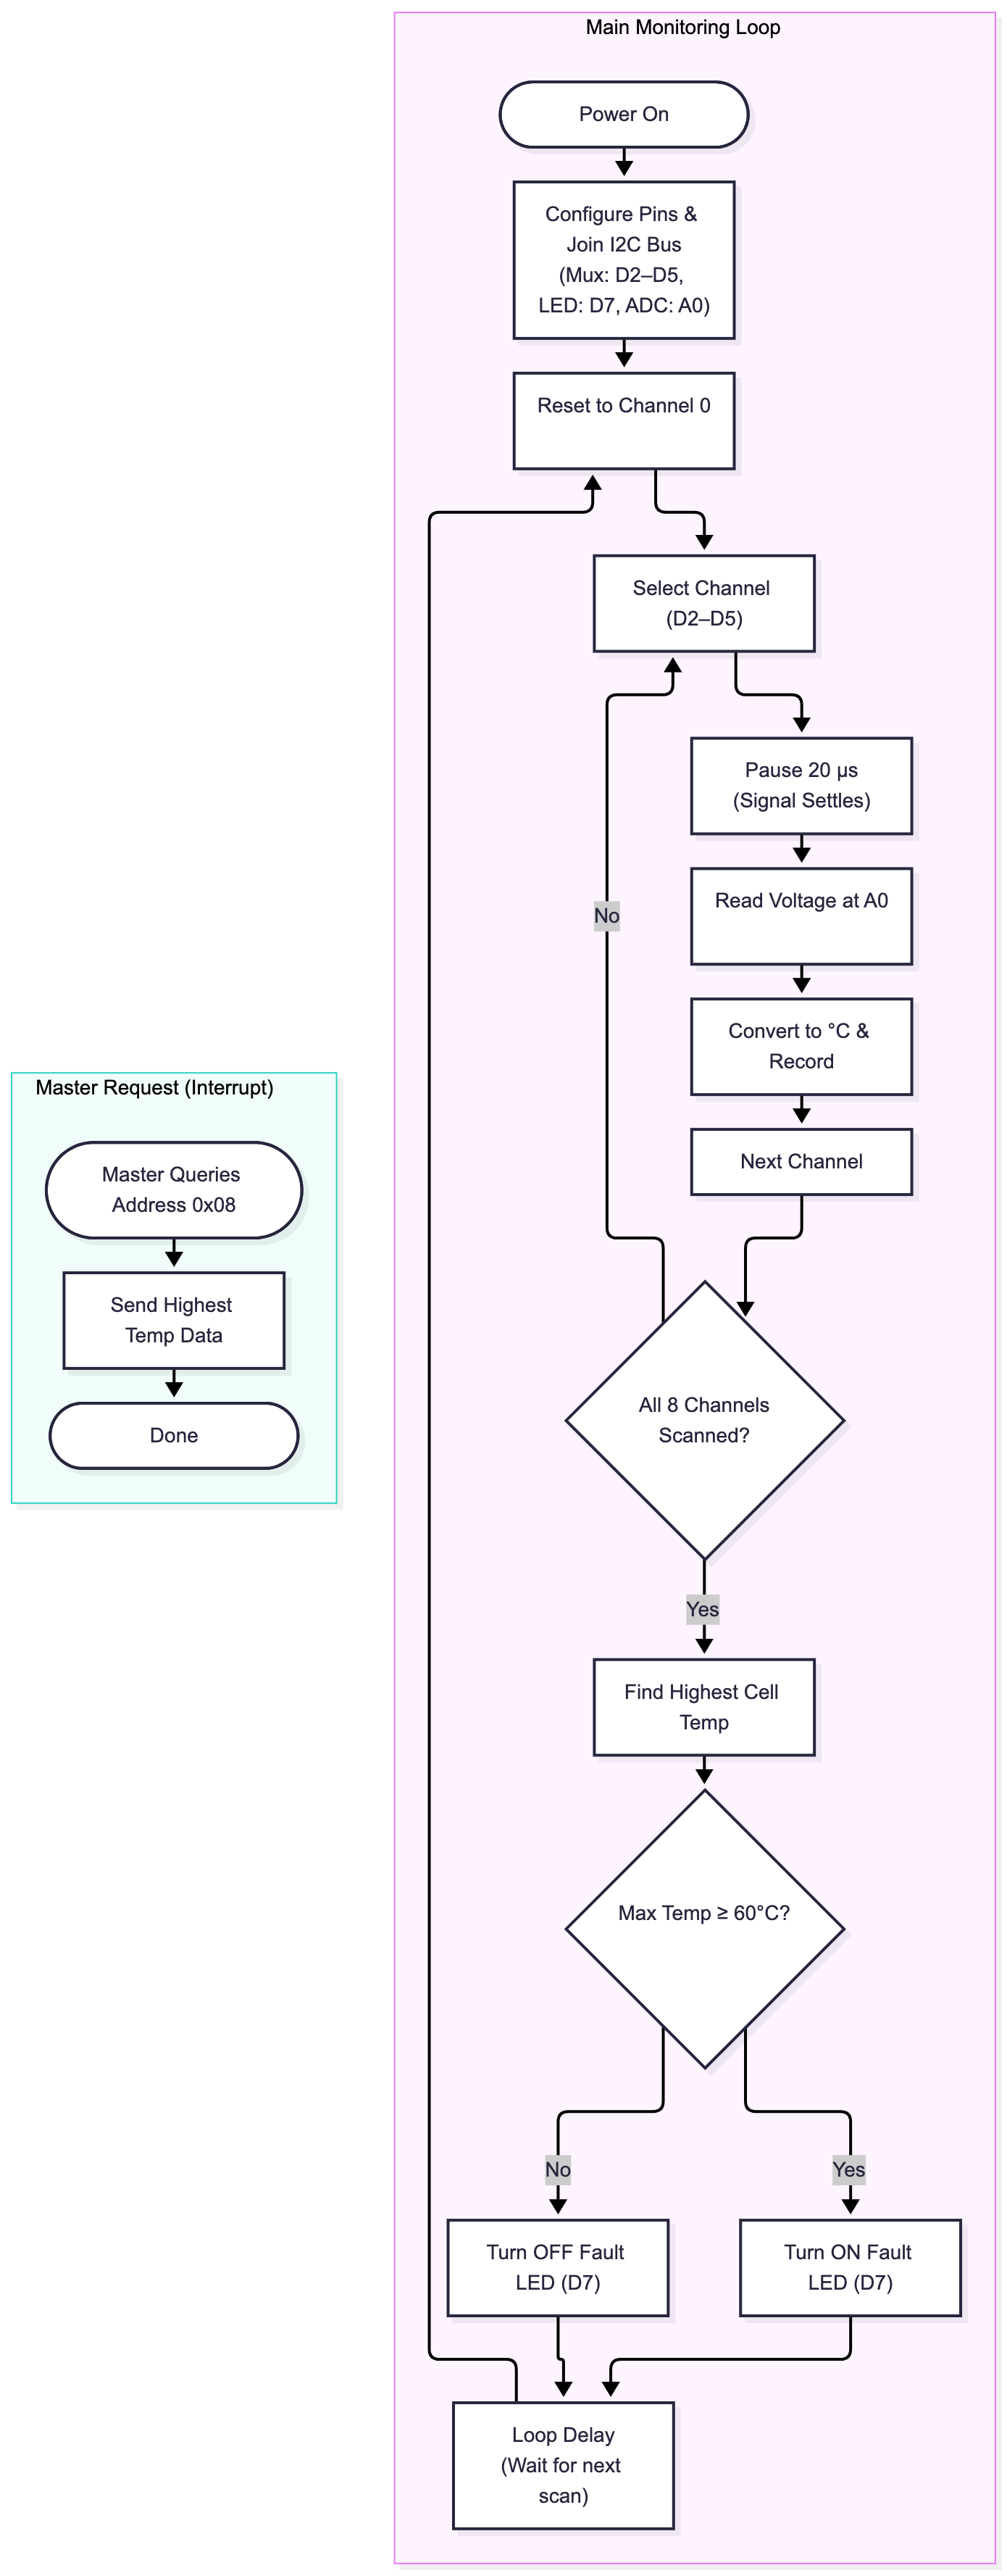
\includegraphics[height=1.0\textheight, width=0.85\linewidth, keepaspectratio]{flowchart.png}
    \caption{Software Flowchart}
    \label{fig:firmware_flowchart}
\end{figure}

The core execution loop performs the following operations:
\begin{enumerate}
    \item Iterates sequentially through channels 0 to 7 using the binary addresses from the select pins
    \item Pauses for an explicit interval ($20\,\mu\text{s}$) to discharge/charge front-end capacitance before sampling.
    \item Samples the conditioned analog node via \lstinline|analogRead(A0)| and converts the raw 10-bit count into an engineering voltage ($0.0\,\text{V} - 5.0\,\text{V}$).
    \item Maps the measured voltage to temperature ($^\circ\text{C}$) based on the Enepaq sensor's temperature and voltage mapping datasheet.
    \item Evaluates cell temperatures against $60^\circ\text{C}$ critical limit, asserting the fault LED on pin \lstinline|D7| if overheating is detected.
    \item Stores the maximum pack temperature to prepare for for I2C request
\end{enumerate}

\subsection{Pin Mapping and Peripheral Allocation}
To match the schematic in Figure~\ref{fig:arduino_temp_sensor_v2}, the hardware-to-software pin definitions are established as constants prior to compilation:

\begin{table}[H]
\centering
\caption{Microcontroller Pin Allocation}
\label{tab:pinout}
\begin{tabular}{llll}
\toprule
\textbf{Constant Name} & \textbf{Nano Pin} & \textbf{Direction} & \textbf{Hardware Functional Description} \\
\midrule
\lstinline|muxSIG|   & A0 & Input  & Conditioned analog voltage from multiplexer op-amp stage \\
\lstinline|muxS0|    & D2 & Output & Binary address select line: Bit 0 ($2^0$) \\
\lstinline|muxS1|    & D3 & Output & Binary address select line: Bit 1 ($2^1$) \\
\lstinline|muxS2|    & D4 & Output & Binary address select line: Bit 2 ($2^2$) \\
\lstinline|muxS3|    & D5 & Output & Binary address select line: Bit 3 ($2^3$) \\
\lstinline|faultLED| & D7 & Output & Over-temperature visual indicator LED \\
\lstinline|SDA|      & A4 & Bidirectional & I2C Data line (configured automatically via \lstinline|Wire.h|) \\
\lstinline|SCL|      & A5 & Input  & I2C Clock line (configured automatically via \lstinline|Wire.h|) \\
\bottomrule
\end{tabular}
\end{table}

\begin{lstlisting}[language=C++, caption={Pin definitions}, label={lst:pin_defs}]
#include <Wire.h>
//Defiing all of our pins here 

Signal Pin from multiplexer to the Arduino
const int muxSIG = A0; 

Pins that will select what channel to read in binary
const int muxS0 = 2;
const int muxS1 = 3;
const int muxS2 = 4;

  
//Defining address for Arduino as Slave
const byte SLAVE_ADDRESS = 0x08;

\end{lstlisting}

\subsection{Overview of functions}

\subsubsection{Channel Addressing: \lstinline|setMuxChannel|}
The CD74HC4067 requires a 4-bit binary code on pins \lstinline|S0|--\lstinline|S3| to connect one of the 16 analog input channels to the common output pin. Instead of manually iterating through binary, we call this function to input the desired channel we want to read, and then it will convert it to the binary equivalent using Arduino's bit read function.

\begin{lstlisting}[language=C++, caption={setMuxChannel Function}, label={lst:mux_code}]
void setMuxChannel(byte channel)  {
  //Allows you to input an integer and then it converts it into binary for the signal pins to read and select the channel
    digitalWrite(muxS0, bitRead(channel, 0));
    digitalWrite(muxS1, bitRead(channel, 1));
    digitalWrite(muxS2, bitRead(channel, 2));
}
\end{lstlisting}

\subsubsection{Signal Acquisition: \lstinline|readChannelVoltage|}
This function switches the channel, pauses for the signal to stabilize, takes a 10-bit analog sample, and converts the integer output to a floating-point voltage:
\begin{equation}
    V_{\text{measured}} = \text{ADC} \times \left(\frac{5.0\,\text{V}}{1023.0}\right)
\end{equation}

\begin{lstlisting}[language=C++, caption={readChannelVoltage Function}, label={lst:read_voltage}]
float readChannelVoltage(byte channel) {
  setMuxChannel(channel);
  delayMicroseconds(20); 

  int rawADC = analogRead(muxSIG);
  return (rawADC * 5.0f) / 1023.0f; //to scale the value and actually put it within our 0-5 range

}
\end{lstlisting}

\subsubsection{Mapping our voltage readings into temperature values: \lstinline|voltagetoTemperature|}
The Enepaq sensor have a table in the data sheet that map out the voltges readings to actually temperature with a certain range. The formula is yet to be determined, but once implemented the function will be able to take in the float voltage value and return a temperature value. 

\begin{lstlisting}[language=C++, caption={Voltage to Temperature Conversion}, label={lst:v_to_t}]
float voltagetoTemperature(float voltage) {
    //Find the reference values and the formula to convert it
    return 0.0f
}
\end{lstlisting}

\subsubsection{I2C Implementation: \lstinline|requestData|}
When the bus master addresses the slave node 0x08, the hardware triggers the request data function. 

\begin{lstlisting}[language=C++, caption={I2C Slave Transmission Callback}, label={lst:i2c_req}]
void requestData() {
    // Send highest recorded pack temperature as a single byte
    Wire.write(maxTempByte);
}
\end{lstlisting}

\subsection{Architectural Decisions and Design Trade-offs}


\subsubsection{Settling Delay Choice ($20\,\mu\text{s}$)}
\begin{itemize}
    \item \textbf{Context:} Inside the multiplexer, each switch adds about $70\,\Omega$ to $180\,\Omega$ of internal resistance ($R_{\text{ON}}$). This sits right before our input filter stage, which uses a $1\,\text{k}\Omega$ resistor and a $10\,\text{nF}$ capacitor before feeding the signal to the op-amp.
    
    \item \textbf{Alternative Considered:} Reading the ADC right after changing the channel address pins, with zero delay in between.
    
    \item \textbf{Decision \& Rationale:} If we sample immediately, voltage left over on the capacitor from the previous channel will bleed into the new reading. For example. The capacitor needs a moment to charge up to the new voltage level. We can find how long this takes using the circuit's RC time constant:
    \begin{equation}
        \tau = R_{\text{total}} \times C \approx (1000\,\Omega + 180\,\Omega) \times 10\,\text{nF} = 11.8\,\mu\text{s}
    \end{equation}
    Waiting $20\,\mu\text{s}$ gives the signal about $1.7\tau$ to settle down, ensuring our ADC reading reflects the true sensor voltage rather than residual charge from the channel before it. Across all 8 channels, this delay is negligible and we would not hinder our target of 1000hz sampling rate. 
\end{itemize}

\subsubsection{Data Typing and Precision (\lstinline|float| vs. \lstinline|int|)}
\begin{itemize}
    \item \textbf{Context:} Choosing the internal representation for voltage readings and temperature calculations.
    \item \textbf{Decision \& Rationale:} With a sensitivity of $-9.5\,\text{mV/}^\circ\text{C}$, a $1^\circ\text{C}$ temperature delta corresponds to a minute voltage change ($\approx 1.94$ ADC counts). Using integer arithmetic would cause severe truncation errors, masking gradual thermal build-up. Single-precision 32-bit floating-point numbers (\lstinline|float|) are used for conversion math to preserve sub-degree precision for over-temperature detection.
\end{itemize}

\section{Verification, Calibration, \& Test Results}

\section{Bill of Materials}

\newpage
\section{Sources} 
\begin{thebibliography}{9}

    \bibitem[]{}\textbf{\large Understanding Our Components}\medskip 
    \bibitem{youtube1} Robotics Back-End, \textit{Arduino Uno - Pins Overview}, YouTube, 2021. Available: \url{https://youtu.be/bniUECtJkeU}

    \bibitem{youtube2} Electronoobs, \textit{Arduino Multiplexor - MUX INPUTS \& OUTPUTS - ANALOG and PWM}, YouTube, 2021. Available: \url{https://youtu.be/Dco6jo9xgAo}

    \bibitem{i2c} Dejan, \textit{How I2C Communication Works?}, HowToMechatronics. Available: \url{https://howtomechatronics.com/tutorials/arduino/how-i2c-communication-works-and-how-to-use-it-with-arduino/}
    
    \bibitem{youtube3} CircuitBread, \textit{Intro to Op-Amps (Operational Amplifiers) | Basic Circuits}, YouTube, 2022. Available: \url{https://youtu.be/fmRHDqcodS4}

    \bibitem{sensor} Temperature Sensor Datasheet. Available: \url{https://enepaq.com/wp-content/uploads/2025/02/Sony-Murata-VTC5A-Li-ion-Battery-Module-With-Temperature-Sensor-Datasheet-.pdf}

    \bibitem[]{}\medskip\medskip\textbf{\large Circuit Basics}\medskip

    \bibitem{youtube4} RimstarOrg, \textit{How to Read a Schematic}, YouTube, 2014. Available: \url{https://youtu.be/_HZ-EQ8Hc8E}

    \bibitem{youtube5} EEVblog, \textit{Playlist on DC Fundamentals}, YouTube, 2017. Available: \url{https://www.youtube.com/show/VLPLZJkSyc12jDY?sbp=KgtZZGJobm1BNE05Z0AB}

    \bibitem[]{}\medskip\medskip\textbf{\large Arduino IDE}\medskip

\end{thebibliography}

\end{document}
